% IIT Roorkee presentation theme for beamer class used in Latex
%
% Manisha Verma, Department of Mathematics,  <mani7dma@iitr.ac.in>
% Sudip Roy, Department of Computer Science and Engineering, <sudiproy.fcs@iitr.ac.in>, <http://faculty.iitr.ac.in/~sudiproy.fcs/>
% Balasubramanian Raman, Department of Computer Science and Engineering, <balarfma@iitr.ac.in>, <https://sites.google.com/site/balaiitr/>
%
% Date: July 23, 2015
% Version 1.0: First public version.

\documentclass[compress]{beamer}

\usetheme{IITR} % To use the theme of IITR for beamer class in Latex

\usepackage{textpos}
\usepackage[utf8]{inputenc}
\usepackage[T1]{fontenc}
\usepackage{helvet}
\usepackage{amsfonts}
\usepackage{amsmath}
\usepackage{amssymb}
\usepackage{tikz, graphicx}
\usetikzlibrary{arrows.meta, positioning}
\usepackage{booktabs}
\setbeamertemplate{navigation symbols}{}
\setbeamertemplate{headline}{}
\setbeamercovered{transparent}
\usebackgroundtemplate{
\includegraphics [width=\paperwidth,height=\paperheight]{slide_bg.png}}
\usepackage{url}

%%%%%%%%%%%%% Title Slide %%%%%%%%%%%%%%%%%
\title{Enabling Onboard Navigation for UAVs in GPS Denied Environments}
\subtitle{MIP400A : B.Tech Project - MidTerm Evaluation}
\author{\small Advika Sinha (23117010) \quad Cherish Puniani (23117042)\\
\small Namay Rohatgi (23119022) \quad Varun R Mallya (23117098)}
\date{{\scriptsize\today} \vspace{3em}}
\institute{Indian Institute of Technology Roorkee}
%%%%%%%%%%%%%%%%%%%%%%%%%%%%%%%%%%%%%%%%%%%
\begin{document}
%%%%%%%%%%%%% Title Slide %%%%%%%%%%%%%%%%%
{\usebackgroundtemplate{
\includegraphics[width=\paperwidth,height=\paperheight]{titleslide_bg.png}}
\begin{frame}[plain,t]
\titlepage
\begin{textblock*}{200mm}(.94\textwidth,-8.75cm)

\includegraphics[height=.98cm]{logo_white.png}
\end{textblock*}
\end{frame}
}
%%%%%%%%%%%%%%%%%%%%%%%%%%%%%%%%%%%%%%%%%%%

%%%%%%%%%%%%% Slide 2: Objectives %%%%%%%%%%%%%%%%%
\section{Objectives}
\begin{frame}[t]{Objectives}
\textbf{Goal:} give a UAV a way to know its own position when GPS/GNSS is unavailable, jammed, or spoofed, using only onboard sensors and physical measurements of its surroundings.
\vspace{0.5em}
\begin{itemize}
\item \textbf{This semester:} get an end-to-end navigation pipeline \emph{working} in simulation (image/data in, position out).
\item \textbf{Next semester (through Apr 2027):} make the pipeline \emph{fast and power-efficient} (FPGA / embedded compute) enough to run onboard real flight hardware.
\end{itemize}
\vspace{0.5em}
\begin{block}{Core approach: Scene-Aided Navigation}
Replace the satellite signal with passive measurements the aircraft can already sense, such as terrain, gravity, magnetic field, and visual scene, matched against a reference map. This turns navigation into a \emph{physical measurement + estimation} problem, much like classical inertial guidance.
\end{block}
\end{frame}
%%%%%%%%%%%%%%%%%%%%%%%%%%%%%%%%%%%%%%%%%%%

%%%%%%%%%%%%% Slide 3: Motivation %%%%%%%%%%%%%%%%%
\section{Motivation}
\begin{frame}[t]{Motivation}
\small
\begin{itemize}
\itemsep 0.4em
\item GNSS is a \textbf{weak radio signal} broadcast from space: it is easily jammed, spoofed, or simply unavailable (urban canyons, mountains, contested airspace, indoors).
\item Autonomous UAVs used in surveying, disaster response, and defense all need to keep flying \emph{when GPS fails}, not just when it works.
\item \textbf{Mechanical perspective:} a UAV is fundamentally a mechanical system in motion. Its onboard IMU already measures physical quantities such as acceleration, rotation, and gravity using mechanical/MEMS sensors. The question this project asks: can these existing physical measurements, combined with a camera, replace the satellite link entirely?
\item \textbf{Precedent:} TERCOM and DSMAC, terrain and scene matching systems developed for Cold-War cruise-missile guidance, proved decades ago that passive, GPS-free navigation using physical terrain data is reliable and flight-proven.
\end{itemize}
\end{frame}
%%%%%%%%%%%%%%%%%%%%%%%%%%%%%%%%%%%%%%%%%%%

%%%%%%%%%%%%% Slide 4: Background of similar work %%%%%%%%%%%%%%%%%
\section{Background of Similar Work}
\begin{frame}[t]{Background of Similar Work}
\small
Passive GPS-denied navigation methods, screened for feasibility on a small UAV:
\vspace{0.3em}
\begin{table}
\centering
\resizebox{\textwidth}{!}{%
\begin{tabular}{@{}llll@{}}
\toprule
\textbf{Method} & \textbf{Physical quantity measured} & \textbf{Passive?} & \textbf{Assessment} \\
\midrule
Terrain matching (TERCOM) & Ground elevation & Yes & Proven, strong candidate\textsuperscript{[4,6]} \\
Visual landmark matching & Camera imagery & Yes & Strong if paired with AI matching\textsuperscript{[1-3,5,7,12,13]} \\
Transformer-based matching & Camera imagery & Yes & SOTA in this niche; motivates our redesign\textsuperscript{[14,15]} \\
Gravity matching & Gravity anomalies & Yes & Promising, needs sensitive sensor\textsuperscript{[8,9]} \\
Gravity-gradient nav. & $\partial g/\partial x,y,z$ & Yes & Very promising, higher precision\textsuperscript{[8,9]} \\
Magnetic anomaly nav. & Magnetic field & Yes & Useful in mountainous terrain\textsuperscript{[10,11]} \\
Quantum inertial sensing & Acceleration / rotation & Yes & No map needed; pure mechanics \\
Wi-Fi / cellular / RF & Radio signal strength & No & Rejected: unavailable at altitude \\
\bottomrule
\end{tabular}}
\end{table}
\vspace{0.3em}
\textbf{Existing implementations reviewed:} VGG16\textsuperscript{[1]} and CLIP-based\textsuperscript{[2,3,7]} deep feature matching of drone frames to satellite tiles (sub-3--7\,m RMSE)\textsuperscript{[2,4]}, classical SIFT/ORB feature matching\textsuperscript{[5]}, terrain-weighted optimization against DEM maps\textsuperscript{[4,6]}.
\end{frame}
%%%%%%%%%%%%%%%%%%%%%%%%%%%%%%%%%%%%%%%%%%%

%%%%%%%%%%%%% Slide 5: Proposed work %%%%%%%%%%%%%%%%%
\section{Proposed Work}
\begin{frame}[t]{Proposed Work}
\begin{center}
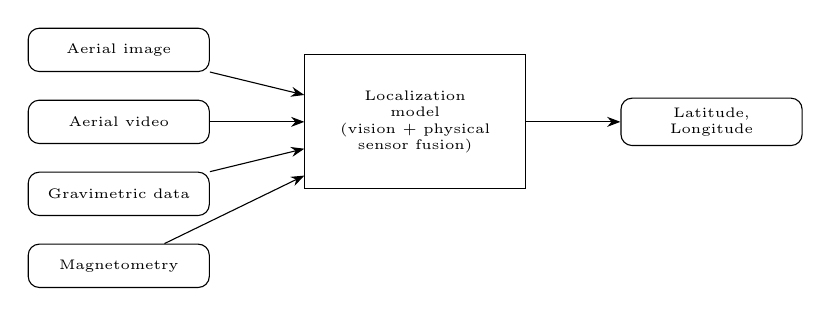
\begin{tikzpicture}[
  node distance=3.5mm and 6mm,
  io/.style={draw, rounded corners, minimum height=0.55cm, minimum width=2.3cm, align=center, font=\tiny},
  model/.style={draw, minimum height=1.7cm, minimum width=2.8cm, align=center, font=\tiny},
  ->, >=Stealth
]
\node[io] (img) {Aerial image};
\node[io, below=of img] (vid) {Aerial video};
\node[io, below=of vid] (grav) {Gravimetric data};
\node[io, below=of grav] (mag) {Magnetometry};
\node[model, right=of vid, xshift=6mm] (model) {Localization\\model\\(vision + physical\\sensor fusion)};
\node[io, right=of model, xshift=6mm] (out) {Latitude,\\Longitude};
\draw (img) -- (model);
\draw (vid) -- (model);
\draw (grav) -- (model);
\draw (mag) -- (model);
\draw (model) -- (out);
\end{tikzpicture}
\end{center}
\vspace{0.1em}
\begin{itemize}
\footnotesize
\itemsep 0.2em
\item \textbf{Current phase (no drone hardware yet):} feed pre-recorded aerial imagery into the pipeline to validate feasibility before committing to flight tests.
\item \textbf{Baseline validated:} replicated the reference implementation\textsuperscript{[1]} in simulation; measured accuracy matches the numbers reported in the paper.
\item \textbf{Current direction:} redesign the localization backbone as a \textbf{transformer-based} model in place of the paper's CNN features (architecture on next slide), then extend it with multimodal sensor fusion.
\end{itemize}
\end{frame}
%%%%%%%%%%%%%%%%%%%%%%%%%%%%%%%%%%%%%%%%%%%

%%%%%%%%%%%%% Slide 5b: Proposed Model Architecture %%%%%%%%%%%%%%%%%
\section{Proposed Model Architecture}
\begin{frame}[t]{Proposed Model Architecture}
\footnotesize
\begin{enumerate}
\itemsep 0.2em
\item \textbf{Data:} aerial images paired with high-precision ground-truth coordinates (from the replicated baseline's flight/simulation data).
\item \textbf{Stage 1 --- vision backbone:} a transformer-based encoder replaces the reference paper's VGG16 features\textsuperscript{[1]}, regressing image $\rightarrow$ coordinates directly.
\item \textbf{Stage 2 --- multimodality:} fuse IMU, magnetometer, and gravimeter (accelerometer) vectors into the transformer alongside the visual stream; train end-to-end for high-precision localization.
\end{enumerate}
\vspace{0.4em}
\begin{center}
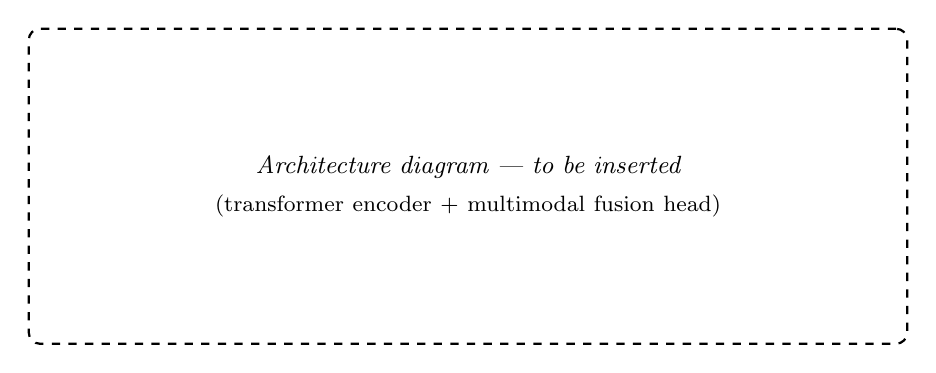
\begin{tikzpicture}
\node[draw, dashed, thick, rounded corners, minimum width=0.92\linewidth, minimum height=4.0cm, align=center, font=\itshape\small, text width=0.8\linewidth]
  {Architecture diagram --- to be inserted\\[0.3em]\normalfont\footnotesize (transformer encoder + multimodal fusion head)};
\end{tikzpicture}
\end{center}
\end{frame}
%%%%%%%%%%%%%%%%%%%%%%%%%%%%%%%%%%%%%%%%%%%

%%%%%%%%%%%%% Slide 6: Timeline %%%%%%%%%%%%%%%%%
\section{Timeline of the Work}
\begin{frame}[t]{Timeline of the Work}
\begin{block}{Phase 1: Now to Nov 2026 (this semester)}
Reference implementation replicated and validated (done); redesign the localization backbone as a transformer model and extend it with multimodal fusion (IMU, magnetometer, gravimeter); get an end-to-end simulated pipeline (aerial image $\rightarrow$ position estimate) working.
\end{block}
\begin{block}{Phase 2: Jan 2027 to Apr 2027}
Optimize the model for speed and power efficiency on FPGA, extending our lab project from last semester which conclusively showed FPGAs are highly power-efficient for this class of computation; integrate onto embedded flight hardware for a physical UAV test.
\end{block}
\end{frame}
%%%%%%%%%%%%%%%%%%%%%%%%%%%%%%%%%%%%%%%%%%%

%%%%%%%%%%%%% References %%%%%%%%%%%%%%%%%
\section{References}
\begin{frame}[t]{References (1/2)}
\tiny
\begin{itemize}
\itemsep 0.35em
\item[{[1]}] H.~Goforth and S.~Lucey, \emph{GPS-Denied UAV Localization using Pre-existing Satellite Imagery}, CMU Robotics Institute. \url{https://publications.ri.cmu.edu/gps-denied-uav-localization-using-pre-existing-satelliteimagery} (code: \url{https://github.com/hmgoforth/gps-denied-uav-localization})
\item[{[2]}] \emph{ngps\_flight}: real-time CLIP-style UAV--satellite matching, $\sim$3\,m RMSE on Jetson Orin. \url{https://github.com/snktshrma/ngps_flight}
\item[{[3]}] \emph{CLIP-UAV-localization}: CLIP-based network matching UAV imagery, also recovers heading. \url{https://github.com/codebra721/CLIP-UAV-localization}
\item[{[4]}] \emph{GNSS-Denied-UAV-Geolocalization}: terrain-weighted optimization using satellite maps and DEM data, sub-7\,m. \url{https://github.com/YFS90/GNSS-Denied-UAV-Geolocalization}
\item[{[5]}] \emph{VisionUAV-Navigation}: classical SIFT/ORB hybrid feature detection, no deep learning. \url{https://github.com/sidharthmohannair/VisionUAV-Navigation}
\item[{[6]}] GNSS-denied UAV geolocalization via terrain-weighted constraint optimization, sub-7\,m error, \emph{ScienceDirect}. \url{https://www.sciencedirect.com/science/article/pii/S1569843224006332}
\item[{[7]}] CLIP-based UAV--satellite image matching, also derives heading direction, \emph{ScienceDirect}. \url{https://www.sciencedirect.com/science/article/pii/S2590123025041787}
\end{itemize}
\end{frame}

\begin{frame}[t]{References (2/2)}
\tiny
\begin{itemize}
\itemsep 0.35em
\item[{[8]}] A Review of Key Technologies in Gravity Matching Navigation, \emph{Sensors} (2026). \url{https://www.mdpi.com/1424-8220/26/13/4208}
\item[{[9]}] Gravity-Aided Navigation Using Viterbi Map Matching Algorithm. \url{https://arxiv.org/abs/2204.10492}
\item[{[10]}] Absolute Positioning Using the Earth's Magnetic Anomaly Field. \url{https://doi.org/10.1002/navi.138}
\item[{[11]}] MagNav-Based Navigation Simulation Using Magnetic Anomaly Maps for GPS-Denied Environments. \url{https://doi.org/10.5302/J.ICROS.2026.25.0344}
\item[{[12]}] \emph{PCVLabDrone2021}: real-time down-facing camera pipeline with quad-tree map retrieval, tested live. \url{https://github.com/OSUPCVLab/PCVLabDrone2021}
\item[{[13]}] \emph{geolocalization}: dual/Siamese network recognizing same-scene UAV and satellite image pairs. \url{https://github.com/abhinavtripathi95/geolocalization}
\item[{[14]}] X.~Zhu et al., \emph{TransGeo: Transformer Is All You Need for Cross-view Image Geo-localization}, CVPR 2022. \url{https://arxiv.org/abs/2204.00097}
\item[{[15]}] \emph{FSRA}: A Transformer-Based Feature Segmentation and Region Alignment Method for UAV-View Geo-Localization. \url{https://arxiv.org/pdf/2201.09206}
\end{itemize}
\end{frame}
%%%%%%%%%%%%%%%%%%%%%%%%%%%%%%%%%%%%%%%%%%%
\end{document}
